\documentclass[a4paper,twocolumn]{article}

\usepackage[utf8]{inputenc} % set input encoding (not needed with XeLaTeX)

\usepackage{amsmath}

\usepackage[margin=0.8in]{geometry}

\geometry{a4paper}

\ifxetex
  \usepackage{fontspec}
  \usepackage{xunicode}
  \defaultfontfeatures{Mapping=tex-text} % To support LaTeX quoting style
  \setmainfont{Cambria}
\else
\fi

\usepackage{graphicx}
\graphicspath{{gfx/}}

\usepackage{booktabs} 
\usepackage{array}
\usepackage{paralist}
\usepackage{verbatim}
\usepackage{caption}
\usepackage{subcaption}
\usepackage{subfloat}
\usepackage{url}
\usepackage{lscape}
\usepackage{amsmath}
\usepackage{fancyhdr}
\usepackage{pgfplots}
\usepackage{siunitx}
\usepackage{tikz}
\usetikzlibrary{positioning,decorations.pathreplacing,shapes,patterns}
\usepackage[europeanresistors,americaninductors,siunitx]{circuitikz}
\usepackage{amssymb}
\pagestyle{fancy}
\renewcommand{\headrulewidth}{0pt}
\lhead{}\chead{\date{}}\rhead{1006511}


\usepackage[hidelinks]{hyperref}
\usepackage[sort&compress,capitalise,noabbrev]{cleveref}

\usepackage{tabularx}
\newcolumntype{R}{>{\raggedleft\arraybackslash}X}%

\usepackage{setspace}
\singlespacing

% Some macros to make re-spacing a little easier
\usepackage{setspace}
% set to singlespace for normal and doublespace for submission
\newcommand{\customspacing}{doublespace}
\newcommand{\bs}{\begin{\customspacing}}
\newcommand{\es}{\end{\customspacing}}

\let\Contentsline\contentsline
\renewcommand\contentsline[3]{\Contentsline{#1}{#2}{#3}}

\usepackage{url}
\usepackage{eurosym}

\title{ES390 \\ Analogue VLSI \\ JWG}
\author{1006511\\
		Oliver Levett\\
		%School of Engineering,\\
  		%University of Warwick,\\
  		%Coventry,\\
  		%United Kingdom,\\
  		%CV4 7AL\\
  		\href{mailto:o.levett@warwick.ac.uk}{o.levett@warwick.ac.uk}}
\graphicspath{{./resources/}}

\newcommand{\infint}{ \int_{-\infty}^{\infty}}
\begin{document}
	\section{Part 2 - Analogue}
		\subsection{Passive components}
			\subsubsection{Resistors}
				\begin{itemize}
					\item Poly \SIrange{20}{40}{\ohm} per square
					\item N-well \SIrange{2}{4}{\kilo \ohm} per square
				\end{itemize}
			\subsubsection{Capacitors}
				\begin{itemize}
					\item MOS \SIrange{2}{3}{\femto \farad \per \square \micro \meter}.
					Between the poly and diffusion regions
					\item Poly 1/Poly 2 cap  \SIrange{0.8}{1}{\femto \farad \per \square \micro \meter}.
				\end{itemize}
			\subsubsection{Switched caps}
				Alternatively, switched caps can be used as resistors.
				\begin{figure}[ht]
					\centering
					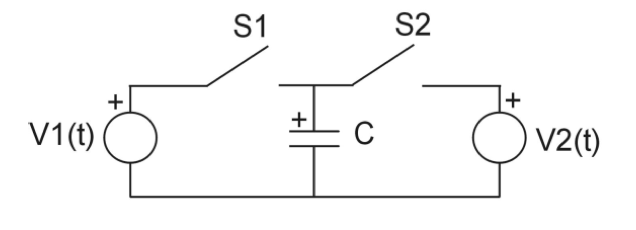
\includegraphics[width=0.45\textwidth]{switched_cap}
				\end{figure}
				\begin{equation}
					R = \frac{T}{C}
				\end{equation}
				where T is the time period of the clock.
		\subsection{Opamp}
			\begin{figure}[ht]
				\centering
				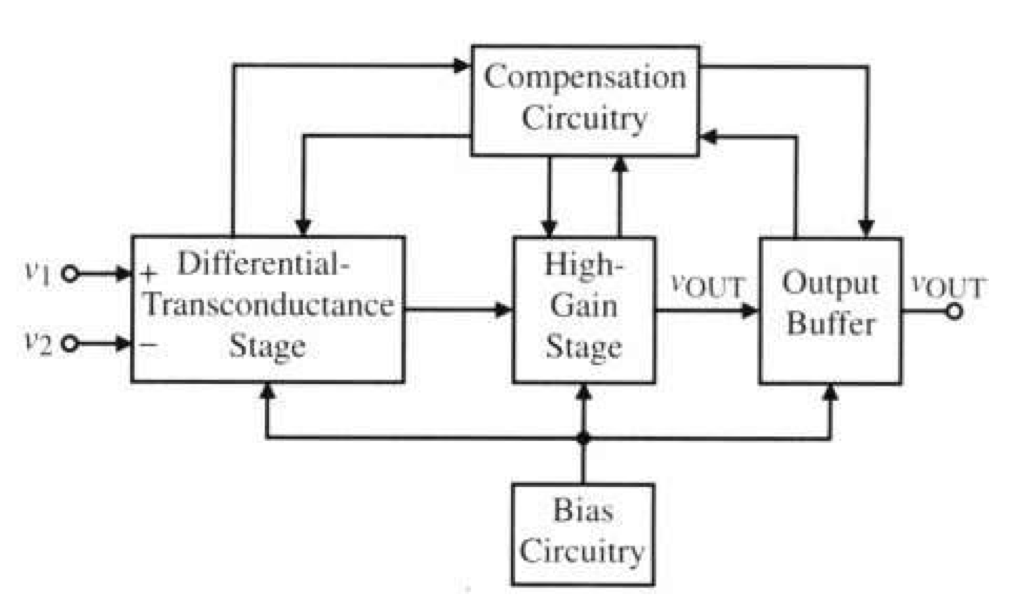
\includegraphics[width=0.45\textwidth]{opamp_parts}
			\end{figure}
			\begin{itemize}
				\item A differential trans-conductance front-end that converts the difference between the input signals 
					v1 and v2 to a current.
				\item A high gain stage that amplifies the input signal
				\item An output buffer stage that is capable of driving a load resistor without reducing
					the gain
				\item Compensation circuitry to improve the frequency characteristics of the amplifier
				\item Bias circuitry to set the DC operating point of the different stages
			\end{itemize}
			
			\begin{figure}[ht]
				\centering
				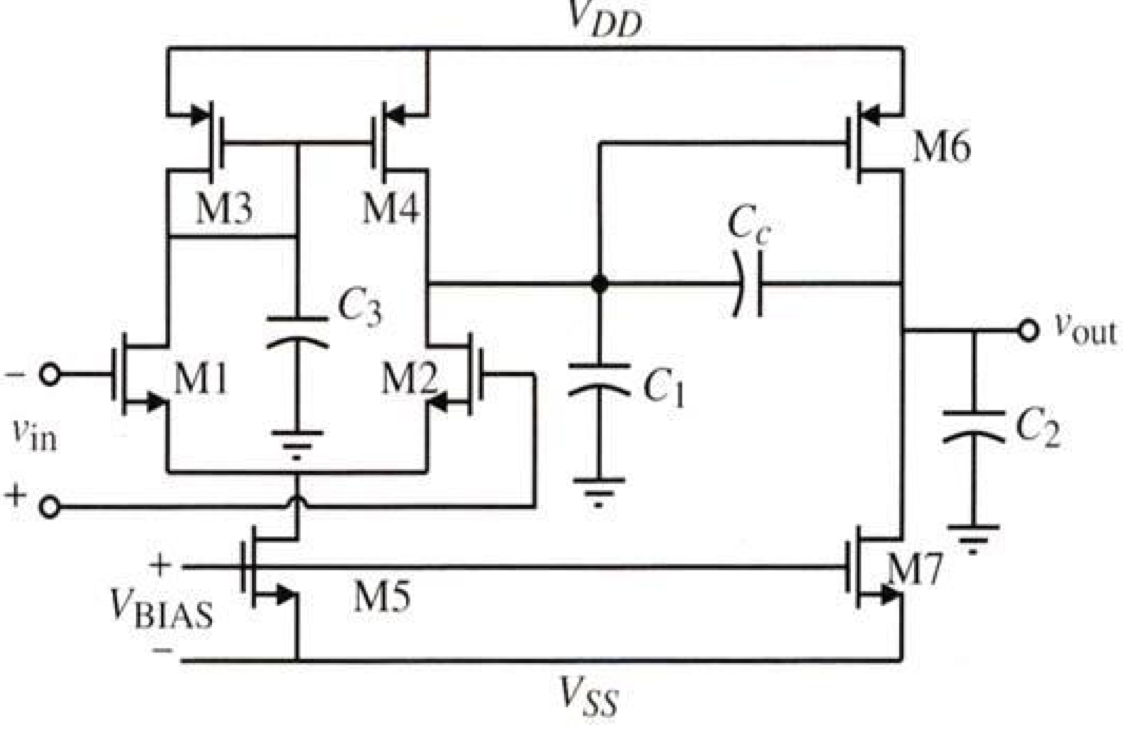
\includegraphics[width=0.45\textwidth]{opamp_schematic}
			\end{figure}
			Miller cap $C_c$ reduces ringing, but should be minimised as it can take a significant proportion of the area.
		
		\subsection{Technologies}
			\subsubsection{SOI vs CMOS}
				Insulated layer below normal CMOS processes
				\begin{table}[ht]
					\centering
					\begin{tabular}{ll}
					Advantages & Disadvantages \\
					\hline
					Better isolation & Cost \\
					Faster & Kink effects \\
					Denser & Floating bodies \\
					Higher temp & Self heating \\
					Lower capacitance & Less robust \\
					\end{tabular}
				\end{table}
			\subsubsection{GaAs}
				\begin{table}[ht]
					\centering
					\begin{tabular}{ll}
					Advantages & Disadvantages \\
					\hline
					& Cost \\
					\end{tabular}
				\end{table}
\end{document}